\documentclass[conference]{IEEEtran}

\usepackage[T1]{fontenc}
\usepackage{amsmath,amssymb}
\usepackage{graphicx}
\usepackage{booktabs}
\usepackage{cite}
\usepackage{url}
\usepackage{xcolor}
\usepackage[section]{placeins}
\usepackage{tikz}
\usetikzlibrary{arrows.meta,positioning}

% Every number below comes from paper/generated/results.tex, which
% paper/make_figures.py builds from the run outputs in runs/.
% Generated by paper/make_figures.py -- do not edit.
\newcommand{\RCurveAllHundred}{0.69M}
\newcommand{\RCurveFirstNinety}{295k}
\newcommand{\RCurveStepZeroMax}{2}
\newcommand{\REvalCommit}{85731ef}
\newcommand{\RFailCollision}{19}
\newcommand{\RFailOther}{1}
\newcommand{\RFailOvershoot}{198}
\newcommand{\RFailTotal}{218}
\newcommand{\RLeadSixCi}{97.8--99.2}
\newcommand{\RLeadSixCollisions}{1}
\newcommand{\RLeadSixHits}{987}
\newcommand{\RLeadSixLaunchRange}{628}
\newcommand{\RLeadSixLaunchRate}{99.9}
\newcommand{\RLeadSixLaunchTime}{20.9}
\newcommand{\RLeadSixRate}{98.7}
\newcommand{\RLeadSweepCi}{96.4--98.3}
\newcommand{\RLeadSweepCollisions}{8}
\newcommand{\RLeadSweepHits}{983}
\newcommand{\RLeadSweepLaunchRange}{650}
\newcommand{\RLeadSweepLaunchRate}{99.2}
\newcommand{\RLeadSweepLaunchTime}{20.9}
\newcommand{\RLeadSweepRate}{97.5}
\newcommand{\ROvershootClosestMax}{130}
\newcommand{\ROvershootClosestMedian}{60}
\newcommand{\ROvershootExampleAspect}{86}
\newcommand{\ROvershootExampleClosest}{60}
\newcommand{\ROvershootExampleId}{SW-b090-h000-r3000-4}
\newcommand{\ROvershootExampleRun}{ppo\_seed2\_sweep}
\newcommand{\ROvershootTimeMax}{3.6}
\newcommand{\ROvershootTimeMedian}{2.8}
\newcommand{\RPpoSixCollisionsMax}{1}
\newcommand{\RPpoSixCollisionsTotal}{2}
\newcommand{\RPpoSixEpisodes}{1000}
\newcommand{\RPpoSixLaunchRange}{993}
\newcommand{\RPpoSixLaunchRate}{100.0}
\newcommand{\RPpoSixLaunchTime}{8.9}
\newcommand{\RPpoSixMax}{99.7}
\newcommand{\RPpoSixMean}{98.98}
\newcommand{\RPpoSixMin}{98.7}
\newcommand{\RPpoSixSd}{0.42}
\newcommand{\RPpoSweepCollisionsMax}{3}
\newcommand{\RPpoSweepCollisionsTotal}{8}
\newcommand{\RPpoSweepEpisodes}{1008}
\newcommand{\RPpoSweepLaunchRange}{993}
\newcommand{\RPpoSweepLaunchRate}{100.0}
\newcommand{\RPpoSweepLaunchTime}{9.0}
\newcommand{\RPpoSweepMax}{98.8}
\newcommand{\RPpoSweepMean}{98.49}
\newcommand{\RPpoSweepMin}{98.1}
\newcommand{\RPpoSweepSd}{0.31}
\newcommand{\RPureSixCi}{96.7--98.5}
\newcommand{\RPureSixCollisions}{0}
\newcommand{\RPureSixHits}{978}
\newcommand{\RPureSixLaunchRange}{996}
\newcommand{\RPureSixLaunchRate}{100.0}
\newcommand{\RPureSixLaunchTime}{9.5}
\newcommand{\RPureSixRate}{97.8}
\newcommand{\RPureSweepCi}{95.7--97.8}
\newcommand{\RPureSweepCollisions}{0}
\newcommand{\RPureSweepHits}{977}
\newcommand{\RPureSweepLaunchRange}{996}
\newcommand{\RPureSweepLaunchRate}{100.0}
\newcommand{\RPureSweepLaunchTime}{9.3}
\newcommand{\RPureSweepRate}{96.9}
\newcommand{\RTrainCommit}{b5c8a49}
\newcommand{\RTrainHours}{1.8}
\newcommand{\RTrainSteps}{1{,}505{,}280}


% Table rows generated by make_figures.py. The primitive \@@input is used
% because LaTeX's \input starts a new cell inside a tabular.
\makeatletter
\newcommand{\tablerows}[1]{\@@input #1 }
\makeatother

\newcommand{\cosata}{\cos\mathrm{ATA}}
\newcommand{\ind}{\mathbf{1}}
\newcommand{\repo}{\url{https://github.com/Akshith-cdr/air-combat-rl-simulation}}

\begin{document}

\title{Learning Pursuit Control for Missile Launch Positioning with PPO in a Kinematic 3D Simulator}

\author{\IEEEauthorblockN{Akshith Veerisetty}
\IEEEauthorblockA{Department of Computer Science and Engineering\\
Indian Institute of Information Technology Sri City, India\\
akshith.v24@iiits.in}}

\maketitle

\begin{abstract}
We study whether a reinforcement learning (RL) policy can learn to fly an aircraft into a missile-launch position against a second aircraft in a kinematic 3D simulator, and whether it does better than classical pursuit guidance. A Proximal Policy Optimization (PPO) policy reads 19 relative-geometry values and outputs pitch, roll, yaw and speed commands. Firing, the launch gate and the proportional-navigation (PN) missile are fixed rules, and the target follows a random patrol without reacting. The same launch gate ($500\le d\le1000$~m and $\cosata>0.95$) is used in training and evaluation. We train five seeds from scratch for \RTrainSteps{} steps each and compare them with pure-pursuit and lead-pursuit controllers on the same episodes: 1,000 episodes from six fixed geometries and a 1,008-episode sweep with the target at twelve bearings around the aircraft and four headings. All five seeds learn the task (mean development hit rate $\ge90\%$ by \RCurveFirstNinety{} steps). On the sweep, PPO scores \RPpoSweepMean\% (seed range \RPpoSweepMin--\RPpoSweepMax\%) against \RLeadSweepRate\% for lead pursuit and \RPureSweepRate\% for pure pursuit; on the six geometries the three controllers lie between \RPureSixRate\% and \RPpoSixMean\%. Nearly every miss is the missile passing the target just outside its 50~m fuse radius, mostly after launches against a crossing target; the remaining failures are collisions. The learned controller therefore matches, and on the all-round sweep slightly exceeds, simple pursuit laws; most of the remaining misses are set by the fixed missile, not by the flight policy.
\end{abstract}

%======================================================================
\section{Introduction}
%======================================================================
Flying one aircraft into a firing position against another is a classic control problem with known solutions: pursuit and proportional-navigation laws steer the velocity vector onto, or ahead of, the line of sight (LOS) \cite{shneydor1998pursuit,zarchan2012guidance}. Deep RL learns a feedback policy from simulated experience instead, and has reached strong results in drone racing \cite{kaufmann2023racing} and simulated dogfights \cite{pope2021hierarchical,li2022msddqn}. Before a learned controller is used in a harder setting, it is worth checking what it adds in a setting where classical laws already work.

This paper asks two narrow questions in a kinematic 3D simulator with a scripted, non-reactive target: (i) can PPO \cite{schulman2017ppo} learn, from scratch and without a curriculum, to bring the aircraft into a fixed launch envelope from any starting bearing; and (ii) how does the result compare with pure and lead pursuit flown in the same environment, under the same launch rule and missile, on the same episodes? Only pursuit flight is learned. The firing rule, the launch gate and the missile guidance are fixed, so the comparison isolates the flight controller.

Our contributions are: a single, reproducible training recipe run with five seeds, with learning curves; a comparison with two classical baselines on two test suites, including a sweep of target bearings and headings all around the aircraft; and an analysis of every failed episode from its recorded trajectory.

%======================================================================
\section{Related Work}\label{sec:related}
%======================================================================
\emph{Model-based maneuvering.} McGrew \emph{et al.} \cite{mcgrew2010adp} computed one-on-one maneuvering policies with approximate dynamic programming. Ure and Inalhan \cite{ure2012ucav} decomposed agile flight into parameterized maneuver modes tracked by sliding-mode controllers on a 6-DOF F-16 model.

\emph{Learning-based air combat.} Li \emph{et al.} \cite{li2022msddqn} let a multi-step double deep Q-network choose among 27 discrete maneuvers of a 6-DOF aircraft. Pope \emph{et al.} \cite{pope2021hierarchical} used hierarchical deep RL for close-range dogfighting. In a small Gymnasium F-16 environment, PPO reached the goal only in some trials whereas a classical autopilot did so reliably \cite{search2025tunnel}, a reminder that a learned controller should be compared with a classical one.

\emph{Guidance.} Pure pursuit, lead pursuit and PN are standard homing laws \cite{shneydor1998pursuit,zarchan2012guidance}; RL has also been used to learn the guidance law itself \cite{gaudet2020intercept}.

\emph{Where this work fits.} Our setting is deliberately simpler than these studies: kinematic aircraft, a non-reactive target and a fixed weapon chain. Its purpose is a clean comparison between a learned and a classical pursuit controller, using PPO from Stable-Baselines3 \cite{raffin2021sb3}.

%======================================================================
\section{Problem Formulation}\label{sec:problem}
%======================================================================
\emph{Task.} Our aircraft carries one guided missile. The target follows a seeded random waypoint patrol, carries no weapons and ignores our aircraft. An episode succeeds when our missile scores a simulated proximity hit. Positions are in metres with $+z$ up, and the simulation advances in fixed steps of $\Delta t=0.05$~s.

\emph{Geometry.} Let $\mathbf{r}=\mathbf{p}_e-\mathbf{p}_o$ be the target position relative to our aircraft, $d=\|\mathbf{r}\|$ the range and $\mathbf{v}_o$ our velocity. Alignment is measured by
\begin{equation}
c=\cosata=\frac{\mathbf{v}_o\cdot\mathbf{r}}{\|\mathbf{v}_o\|\,\|\mathbf{r}\|}.
\end{equation}
The \emph{bearing} of the target is measured clockwise from our nose (0 = ahead, 180$^\circ$ = behind), and the target's \emph{relative heading} is its compass heading minus ours.

\emph{Observation.} The policy sees the 19 values in Table~\ref{tab:obs}, read directly from the simulator (no sensor model), standardized with running statistics and clipped to $\pm10$.

\begin{table}[t]
\centering
\caption{Policy observation $o_t\in\mathbb{R}^{19}$ (simulator ground truth).}
\label{tab:obs}
\footnotesize
\setlength{\tabcolsep}{4pt}
\begin{tabular}{@{}rl@{\hspace{8pt}}rl@{}}
\toprule
Idx & Quantity & Idx & Quantity \\
\midrule
0 & airspeed $V$ (m/s) & 11 & alignment $c=\cosata$ \\
1 & altitude $h$ (m) & 12 & relative speed (m/s) \\
2 & velocity--nose angle $\alpha$ & 13 & relative vertical vel. (m/s) \\
3 & load-factor estimate & 14 & range rate $\dot d$ (m/s) \\
4--6 & roll, pitch, yaw (deg) & 15 & LOS bearing error $e_\psi$ (deg) \\
7--9 & relative position $\mathbf{r}$ (m) & 16 & LOS elevation error $e_\theta$ (deg) \\
10 & range $d$ (m) & 17 & lateral relative vel. (m/s) \\
 & & 18 & commanded speed (m/s) \\
\bottomrule
\end{tabular}
\end{table}

\emph{Action.} $a_t=(u_\theta,u_\phi,u_\psi,u_v)\in[-1,1]^4$: pitch, roll and yaw rate commands and a throttle command. The policy has no fire output.

\emph{Launch rule and gate.} Until the missile has left the aircraft, a launch is requested at every step. The gate accepts it only if
\begin{equation}
500~\mathrm{m}\le d_t\le 1000~\mathrm{m}\quad\text{and}\quad c_t>0.95,
\label{eq:gate}
\end{equation}
i.e.\ the velocity is within $18.2^\circ$ of the LOS. The missile is therefore released on the first step at which the aircraft is inside the range band and pointing at the target. Training and evaluation read this gate from the same configuration file, so they cannot differ.

\emph{Episode end.} An episode ends with exactly one outcome: a \emph{hit}; a \emph{collision} (our aircraft within 10~m of the target at any point of a step, checked on the swept relative path); \emph{ground} (our aircraft below $z=0$); a missile that ends without a hit (20~s lifetime, 25~km range, or below $z=-1000$~m); leaving the 10~km chase boundary; or a 2,000-step (100~s) time limit. Only a hit counts as success; a collision is a failure even if the missile later hits.

\emph{Reward.} With the distance outside the band $\epsilon(d)=\max(0,d-1000)+\max(0,500-d)$ and $L_t=1$ until the missile is launched, the per-step reward is
\begin{equation}
\begin{aligned}
r_t ={}& L_t\big(r^{\mathrm{cl}}_t + r^{\mathrm{al}}_t + r^{\mathrm{geo}}_t\big) && \text{(engagement)}\\
&+ 0.5\,r^{V}_t + 0.5\,r^{h}_t + r^{\alpha}_t && \text{(safety)}\\
&+ r^{\mathrm{ev}}_t - 0.01 && \text{(events)}
\end{aligned}
\label{eq:reward}
\end{equation}
with
\begin{align*}
r^{\mathrm{ev}}_t &= 5\,\ind_{\mathrm{launch}} + 100\,\ind_{\mathrm{hit}} - 50\,\ind_{\mathrm{coll}} - 25\,\ind_{\mathrm{bnd}},\\
r^{\mathrm{cl}}_t &= \mathrm{clip}\big((\epsilon(d_{t-1})-\epsilon(d_t))/(250\,\Delta t)\big),\\
r^{\mathrm{al}}_t &= \max(0,r^{\mathrm{cl}}_t)\,\mathrm{clip}_{[0,1]}\big((c_t-0.95)/0.05\big),\\
r^{\mathrm{geo}}_t &= \mathrm{clip}\big((P_t-P_{t-1})/0.1\big),\\
P_t &= \mathrm{clip}_{[0,1]}\big(1-\epsilon(d_t)/500\big)\,(1+c_t)/2,\\
r^{V}_t &= -\mathrm{clip}_{[0,1]}\big((150-V_t)/75\big),\\
r^{h}_t &= -\mathrm{clip}_{[0,1]}\big((250-h_t)/125\big),\\
r^{\alpha}_t &= -\mathrm{clip}_{[0,1]}\big((|\alpha_t|-15^\circ)/30^\circ\big).
\end{align*}
$\mathrm{clip}$ limits to $[-1,1]$ and $\mathrm{clip}_{[0,1]}$ to $[0,1]$; $\ind_{\mathrm{coll}}$ covers both collision and ground. The engagement terms reward moving into the band, closing while aligned, and progress towards an aligned position inside the band. They are switched off after launch, so nothing rewards flying closer to the target while the missile is in flight. The safety terms are zero in normal flight. Equation~\eqref{eq:reward} is a transcription of the function \texttt{reward\_terms} in the released code.

%======================================================================
\section{Method}\label{sec:method}
%======================================================================
\emph{System.} Fig.~\ref{fig:arch} shows how the parts connect. Only the shaded block is learned; the baselines replace it with a fixed controller and leave everything else unchanged.

\begin{figure}[t]
\centering
\resizebox{\columnwidth}{!}{%
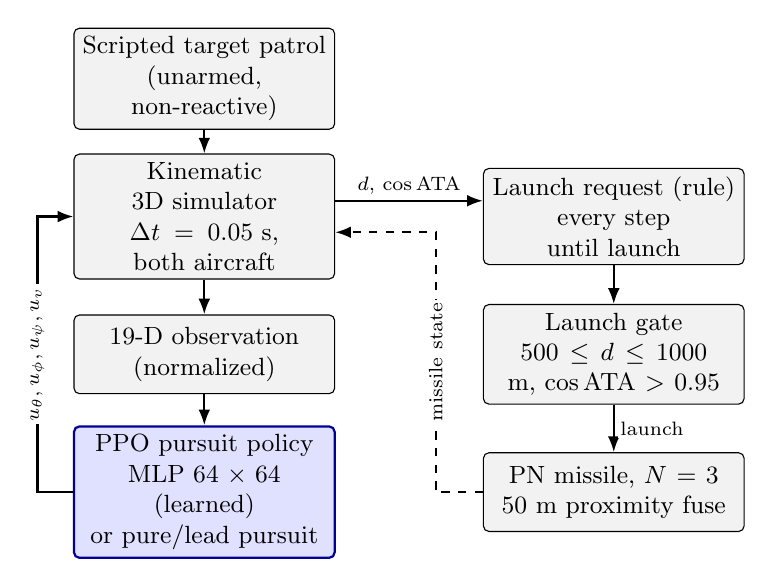
\begin{tikzpicture}[
  box/.style={draw, rounded corners=2pt, align=center, text width=3.1cm, minimum height=10mm, inner sep=3pt, font=\small},
  learned/.style={box, fill=blue!12, draw=blue!60!black, thick},
  rule/.style={box, fill=gray!10},
  arr/.style={-{Latex[length=2mm]}, thick},
  lbl/.style={font=\scriptsize, fill=white, inner sep=1pt}]
\node[rule]    (enemy) at (0, 1.75)  {Scripted target patrol\\(unarmed, non-reactive)};
\node[rule]    (sim)   at (0, 0)     {Kinematic 3D simulator\\$\Delta t=0.05$ s, both aircraft};
\node[rule]    (obs)   at (0,-1.75)  {19-D observation\\(normalized)};
\node[learned] (pi)    at (0,-3.5)   {PPO pursuit policy\\MLP $64\times64$ (learned)\\or pure/lead pursuit};
\node[rule]    (req)   at (5.2, 0)   {Launch request (rule)\\every step until launch};
\node[rule]    (gate)  at (5.2,-1.75){Launch gate\\$500\le d\le1000$ m, $\cosata>0.95$};
\node[rule]    (msl)   at (5.2,-3.5) {PN missile, $N=3$\\50 m proximity fuse};
\draw[arr] (enemy) -- (sim);
\draw[arr] (sim) -- (obs);
\draw[arr] (obs) -- (pi);
\draw[arr] (pi.west) -- ++(-0.45,0) |- node[lbl, pos=0.25, rotate=90]{$u_\theta,u_\phi,u_\psi,u_v$} (sim.west);
\draw[arr] ([yshift=2mm]sim.east) -- node[lbl, above=1pt]{$d$, $\cosata$} ([yshift=2mm]req.west);
\draw[arr] (req) -- (gate);
\draw[arr] (gate) -- node[lbl, right=1pt]{launch} (msl);
\draw[arr, dashed] (msl.west) -- ++(-0.6,0) |- node[lbl, pos=0.25, rotate=90]{missile state} ([yshift=-2mm]sim.east);
\end{tikzpicture}}
\caption{System architecture. The pursuit controller (shaded) is the only part that differs between PPO and the baselines; the target patrol, launch rule, gate and missile guidance are fixed.}
\label{fig:arch}
\end{figure}

\emph{Aircraft model.} Both aircraft use the same kinematic model. Each body rate follows its command with a first-order lag, $\omega_i\leftarrow\omega_i+8\Delta t\,(S_iu_i-\omega_i)$, with $S_{\phi,\theta,\psi}=51.0,\,40.5,\,40.3$~deg/s. Banking beyond $15^\circ$ adds a coordinated turn rate; roll and pitch are limited to $\pm90^\circ$; $u_v$ moves the commanded speed at up to $\pm100$~m/s$^2$, which the actual speed follows with a lag. The velocity direction is pulled towards the nose each step and the position is integrated from it. The model has no gravity and no drag. The target steers towards random waypoints within 1,500~m horizontally and 900~m vertically of its start, re-drawn every 2--5~s, at 140--240~m/s.

\emph{Why a kinematic model.} Our question is geometric: can a controller bring the velocity vector onto the LOS inside a range band, from any starting bearing? That depends on turn rate, speed and their lags, which the model represents, and much less on the energy and stability effects that a 6-DOF model adds. The same model is used by the learned and the classical controllers, so the comparison is fair within it. The absolute hit rates, however, should not be read as predictions for a real aircraft. Moving to a flight-dynamics model such as JSBSim \cite{berndt2004jsbsim}, where gravity, drag and energy management matter, is the main next step (Section~\ref{sec:limits}).

\emph{Missile.} The missile is a point mass launched with our velocity plus 35~m/s along the nose, boosting at 120~m/s$^2$ for 3~s up to 650~m/s. Its commanded acceleration is
\begin{equation}
\mathbf{a}_M = N\,V_c\,(\boldsymbol\Omega\times\hat{\mathbf{u}}),\qquad N=3,
\label{eq:pn}
\end{equation}
where $\boldsymbol\Omega$ is the LOS rate, $V_c$ the closing speed and $\hat{\mathbf{u}}$ the missile's flight direction, capped at 250~m/s$^2$ and $120^\circ$/s and integrated in 0.01~s substeps with the true target state. A hit is scored when the swept paths of missile and target pass within 50~m.

\emph{PPO agent and training.} The policy is a Stable-Baselines3 \cite{raffin2021sb3} actor--critic with separate two-layer, 64-unit tanh networks; the actor outputs the mean of a 4-D Gaussian with a state-independent spread. Every run starts from random weights in the final task: there is no curriculum, warm start or earlier stage. Each run trains for \RTrainSteps{} steps on 3 parallel environments with rollouts of $3\times2{,}048$ steps, minibatch 256, 10 epochs, learning rate $3\cdot10^{-4}$, $\gamma=0.995$, GAE $\lambda=0.95$ \cite{schulman2016gae}, clip range 0.2, no entropy bonus, and observation and reward normalization. Each training episode draws a new geometry: target bearing uniform over $360^\circ$, range 1.5--5~km, relative heading uniform over $360^\circ$, altitude 1.0--2.2~km, altitude difference $\pm500$~m, our speed 160--260~m/s and target speed 140--240~m/s. We train seeds 1--5 with identical settings (about \RTrainHours~h each on one CPU core). Evaluation uses the mean action.

\emph{Baselines.} Both baselines read the true state and output the same four commands. \emph{Pure pursuit} aims the velocity vector at the target; \emph{lead pursuit} aims it at $\mathbf{p}_e+\mathbf{v}_e t_{go}$ with $t_{go}=d/V_c$ clipped to 0--5~s \cite{shneydor1998pursuit}. For an aim-point heading error $e$ (deg), the bank command is $1.5e$ limited to $\pm75^\circ$, the yaw command $-e/20$ and the pitch command steers the nose to the aim-point elevation (limited to $\pm45^\circ$). Speed is held at the target's speed plus $0.1(d-750)$~m/s (limited to $\pm200$~m/s, at least 160~m/s), so the aircraft closes when far and matches the target near the middle of the band. The gains were set once by hand and not tuned on the test suites.

%======================================================================
\section{Experimental Setup}\label{sec:setup}
%======================================================================
\emph{Test suites.} (1) \emph{Six geometries}: the 1,000-episode protocol of our earlier report, with the same episode seeds and seed-to-geometry assignment. Our aircraft starts at $(0,0,1000)$~m, heading $0^\circ$, 150~m/s; the target starts at one of six positions 2.5--4.3~km away within $29^\circ$ of the nose (Table~\ref{tab:scen}). (2) \emph{All-round sweep}: target bearing $0,30,\dots,330^\circ$, relative heading $0,90,180,270^\circ$, range 1.5, 3 or 4.5~km, each combination with 7 simulator seeds (1,008 episodes); both aircraft at 1.5~km altitude, 200 and 190~m/s. Episodes with the same geometry differ only in the target's random waypoints. Every controller is flown on exactly the same episodes.

\emph{Development set.} During training, each run is flown every 98,304 steps on 48 episodes (one per bearing and heading of the sweep at 3~km, with separate simulator seeds) to obtain learning curves. These episodes share geometries with the sweep but not seeds, and they were not used to choose any setting.

\emph{Metrics.} Hit rate (with 95\% Wilson intervals \cite{wilson1927} for single runs, and mean, standard deviation and range over the five seeds for PPO), collisions, the time and range at launch, and the category of each failure.

\emph{Reproducibility.} Training and evaluation refuse to run from uncommitted code, and every checkpoint and result stores the git commit, the full task and PPO configuration and the package versions. The policies were trained at commit \texttt{\RTrainCommit} and evaluated at commit \texttt{\REvalCommit} (which only adds diagnostic fields; hit counts are unchanged). All commands and artifact names are listed in the Appendix. In revising this work we also corrected two initialization errors of the earlier simulator, where the target started with its nose mirrored relative to its flight direction and banked at $90^\circ$.

%======================================================================
\section{Results}\label{sec:results}
%======================================================================
\begin{figure}[t]
\centering
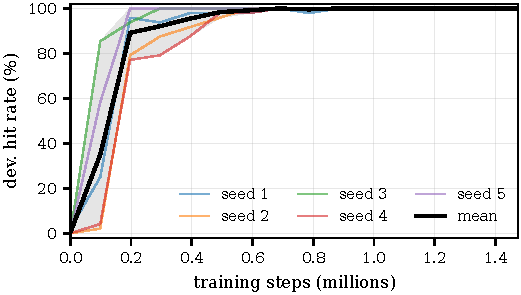
\includegraphics[width=\columnwidth]{figures/fig_learning.pdf}
\caption{Learning curves: hit rate on the 48-episode development set versus training steps for five seeds trained from scratch; black line = mean, grey band = min--max.}
\label{fig:learning}
\end{figure}

\emph{Learning.} Fig.~\ref{fig:learning} shows that every seed starts near zero (at most \RCurveStepZeroMax\% at step 0) and learns the task. The mean development hit rate passes 90\% at \RCurveFirstNinety{} steps and all five seeds reach 100\% by \RCurveAllHundred{} steps. Seeds differ mainly in how quickly they leave the early phase in which the aircraft flies into the ground or leaves the boundary. The development set saturates, so it cannot show changes after that point; the test suites below are the measure of the final policies.

\begin{figure*}[t]
\centering
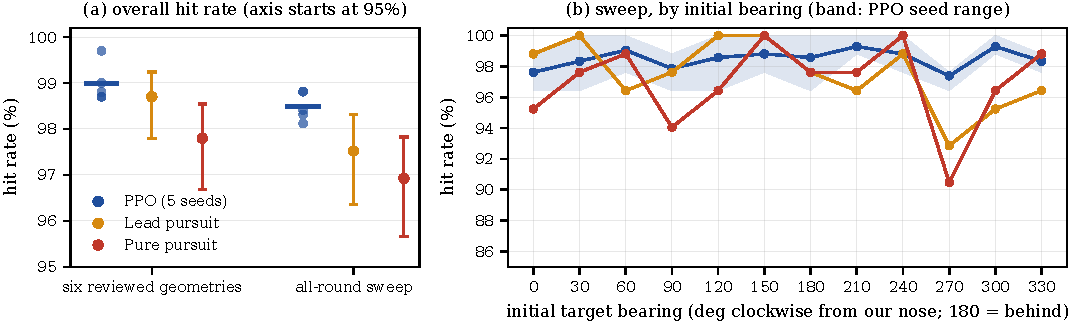
\includegraphics[width=\textwidth]{figures/fig_comparison.pdf}
\caption{PPO versus the baselines on identical episodes. (a) Hit rate on both suites: PPO seeds as dots with their mean as a bar; baselines with 95\% Wilson intervals. The vertical axis starts at 95\%. (b) Sweep hit rate per initial bearing (84 episodes per sector per controller); the shaded band is the range over the five PPO seeds.}
\label{fig:comparison}
\end{figure*}

\begin{table}[t]
\centering
\caption{Hit rate (\%) of each controller; PPO: mean $\pm$ s.d. (range) over 5 seeds, baselines: rate (95\% CI). Collisions per run and median launch time and range are for the sweep.}
\label{tab:comparison}
\footnotesize
\setlength{\tabcolsep}{2.5pt}
\resizebox{\columnwidth}{!}{%
\begin{tabular}{@{}lccccc@{}}
\toprule
Controller & Six geometries & Sweep & Coll. & $t_\mathrm{L}$ (s) & $d_\mathrm{L}$ (m) \\
\midrule
\tablerows{generated/tab_comparison.tex}
\bottomrule
\end{tabular}}
\end{table}

\emph{Comparison with the baselines.} Table~\ref{tab:comparison} and Fig.~\ref{fig:comparison}(a) give the main result. On the all-round sweep, every PPO seed scores higher than both baselines: PPO \RPpoSweepMean\% (range \RPpoSweepMin--\RPpoSweepMax\%), lead pursuit \RLeadSweepRate\% (CI \RLeadSweepCi\%), pure pursuit \RPureSweepRate\% (CI \RPureSweepCi\%). The margin is small: the PPO mean is 1.0 points above lead pursuit and 1.6 above pure pursuit, and the worst seed is 0.6 points above lead pursuit. On the six geometries the controllers are closer: PPO \RPpoSixMean\% (range \RPpoSixMin--\RPpoSixMax\%), lead pursuit \RLeadSixRate\%, pure pursuit \RPureSixRate\%; the PPO seed range overlaps lead pursuit's interval. PPO and pure pursuit launched in every episode of both suites; lead pursuit launched in \RLeadSixLaunchRate\% and \RLeadSweepLaunchRate\% of episodes (see collisions below).

\emph{By starting bearing.} No bearing sector is hard for any controller (Fig.~\ref{fig:comparison}(b)): targets beside or behind the aircraft are reached as reliably as targets ahead. The lowest sector rates belong to the baselines (pure pursuit at $90^\circ$ and $270^\circ$, lead pursuit at $270^\circ$--$300^\circ$); the PPO seed band stays above about 96\% in every sector. With 84 episodes per sector, differences of a few points are within noise.

\begin{table}[t]
\centering
\caption{The six reviewed geometries: target start position (our aircraft at $(0,0,1)$~km, heading $0^\circ$, 150~m/s), range $d_0$, bearing $\beta_0$, target heading $\psi_e$ and speed $V_e$, and hit rate (\%) per controller (PPO pooled over 5 seeds).}
\label{tab:scen}
\footnotesize
\setlength{\tabcolsep}{2pt}
\begin{tabular}{@{}lccrrrccc@{}}
\toprule
ID & Target (km) & $d_0$ (km) & $\beta_0$ ($^\circ$) & $\psi_e$ ($^\circ$) & $V_e$ & PPO & Lead & Pure \\
\midrule
\tablerows{generated/tab_scenarios.tex}
\bottomrule
\end{tabular}
\end{table}

\emph{Launch timing and the band.} Most launches happen just inside the outer edge of the band (median \RPpoSweepLaunchRange~m for PPO, \RPureSweepLaunchRange~m for pure pursuit). This is a property of the rule, not evidence of skill: the gate fires on the first aligned step inside the band, so any controller that approaches while pointing at the target launches near 1,000~m. Lead pursuit is the exception: it aims ahead of the target, so its velocity is often more than $18^\circ$ off the LOS and it launches later and closer (median \RLeadSweepLaunchTime~s and \RLeadSweepLaunchRange~m against \RPpoSweepLaunchTime~s for PPO). The earlier hypothesis that the learned pursuit ``naturally passes through the band'' is therefore true but not specific to learning: pure pursuit does the same.

\begin{table}[t]
\centering
\caption{Failures per run by category (PPO: mean over 5 seeds).}
\label{tab:failures}
\footnotesize
\setlength{\tabcolsep}{3pt}
\begin{tabular}{@{}lcccccc@{}}
\toprule
 & \multicolumn{3}{c}{Six geometries} & \multicolumn{3}{c}{Sweep} \\
\cmidrule(lr){2-4}\cmidrule(lr){5-7}
Controller & Oversh. & Coll. & Other & Oversh. & Coll. & Other \\
\midrule
\tablerows{generated/tab_failures.tex}
\bottomrule
\end{tabular}
\end{table}

\begin{figure}[t]
\centering
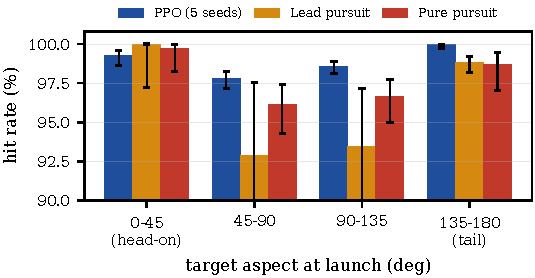
\includegraphics[width=\columnwidth]{figures/fig_aspect.pdf}
\caption{Hits per launch by the target's aspect at launch (angle between the target's velocity and the line from the target to our aircraft; 0 = head-on, 180 = tail), pooled over both suites, with 95\% Wilson intervals. The vertical axis starts at 90\%.}
\label{fig:aspect}
\end{figure}

\begin{figure}[t]
\centering
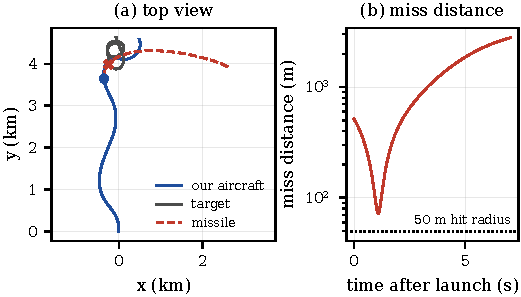
\includegraphics[width=\columnwidth]{figures/fig_overshoot.pdf}
\caption{A typical overshoot miss (\ROvershootExampleRun, \ROvershootExampleId; the failure with the median miss distance among PPO sweep misses). (a) Top view from launch (dot) to 6~s after the closest approach ($\times$). (b) Missile--target distance after launch; the missile passes \ROvershootExampleClosest~m from the target, outside the 50~m radius, and then diverges.}
\label{fig:overshoot}
\end{figure}

\emph{Why episodes fail.} We recorded the full trajectory of every failed episode and classified all \RFailTotal{} of them (Table~\ref{tab:failures}). \RFailOvershoot{} are \emph{missile overshoots}: the missile passed the target at \ROvershootClosestMedian~m (median; at most \ROvershootClosestMax~m), just outside its 50~m fuse radius, \ROvershootTimeMedian~s after launch (at most \ROvershootTimeMax~s), and could not turn back before its 20~s lifetime or the floor ended it (Fig.~\ref{fig:overshoot}). \RFailCollision{} are collisions, which differ by controller: all 10 PPO collisions happened \emph{after} launch, when the aircraft kept pursuing while its missile was in flight, whereas all 9 lead-pursuit collisions happened \emph{before} launch, when the aircraft, aiming ahead of the target, flew into it without its velocity ever coming within $18^\circ$ of the LOS inside the band. Pure pursuit had none. The single remaining failure is a lead-pursuit missile whose closest approach was 152~m, just outside our 150~m near-miss threshold. Overshoots concentrate in launches against a crossing target (Fig.~\ref{fig:aspect}): at $45$--$135^\circ$ aspect the LOS rotates fastest, and the rate- and acceleration-limited PN missile swings past. Head-on launches almost never miss, and neither do tail launches by PPO (1 miss in 2,207) or pure pursuit (5 in 387). Lead pursuit launches mostly from the tail but at shorter range, and misses 1.2\% of those. Most of the remaining gap to 100\% is therefore a property of the fixed missile, which the flight controller influences only through the geometry at launch.

%======================================================================
\section{Discussion}\label{sec:discussion}
%======================================================================
PPO learned, from scratch and in one run per seed, a pursuit controller that reaches the launch envelope from any starting bearing. Measured against classical pursuit on identical episodes, it is as good on the six reviewed geometries and slightly better on the all-round sweep, where every seed beats both baselines (by 0.6 to 1.9 points). The difference is consistent across seeds but small, and part of it may come from untuned baseline gains; a stronger, tuned baseline could close it. Lead pursuit's higher collision count and later launches show that the classical controllers also make visible trade-offs that the learned policy does not share in this setting. Because a simple pure-pursuit law already reaches about 97\%, this task does not by itself demonstrate a need for RL; what it shows is that the learned controller is competitive with classical guidance and that the training recipe is reliable across seeds.

%======================================================================
\section{Limitations and Future Work}\label{sec:limits}
%======================================================================
\emph{Limitations.} Only the flight controller is learned; firing, the gate and the PN missile are fixed. The target is scripted, unarmed and non-reactive. The aircraft model is kinematic (no gravity or drag) and sensing is perfect; a hit is a 50~m proximity event. The development set saturates by \RCurveAllHundred{} steps, so later training progress is not measured. The baselines use hand-set gains, and both test suites use the same altitude band for both aircraft.

\emph{Future work.} (i) Move to a flight-dynamics model such as JSBSim \cite{berndt2004jsbsim}, where energy management could separate learned and classical controllers more clearly; (ii) a post-launch separation reward to remove PPO's few collisions; (iii) a target that turns away when it detects a launch, where launch timing and aspect matter more; (iv) learning the firing decision, using the aspect dependence of Fig.~\ref{fig:aspect}; and (v) a two-sided engagement in which both aircraft are armed.

%======================================================================
\section{Conclusions}\label{sec:conclusion}
%======================================================================
We trained a PPO pursuit controller from scratch with five seeds in a kinematic 3D simulator, using the same launch gate in training and evaluation, and compared it with pure and lead pursuit on 2,008 identical episodes per controller. All seeds learned the task. PPO reached \RPpoSweepMean\% on an all-round sweep of starting bearings (lead pursuit \RLeadSweepRate\%, pure pursuit \RPureSweepRate\%) and matched the baselines on six fixed geometries. Nearly all failures are missile overshoots, mostly against crossing targets; PPO's few collisions occur after launch, while it keeps pursuing. The learned controller is competitive with, and slightly better than, simple pursuit guidance in this setting; showing a clear advantage for RL will require a harder task, such as a reactive target or a full flight-dynamics model.

\section*{Acknowledgement}
We thank Dr. Piyush Joshi, Indian Institute of Information Technology Sri City, for guidance and supervision of this project. The work used the open-source Stable-Baselines3, PyTorch and Panda3D \cite{goslin2004panda3d} libraries.

\appendix
\section*{Appendix: Code and Artifacts}
Code, configurations, results and this paper are at \repo. The pipeline is in \path{pursuit/}: \path{config.py} (gate, collision radius, reward constants), \path{env.py} (environment and reward \eqref{eq:reward}), \path{scenarios.py} (training distribution and test suites), \path{baselines.py}, \path{train.py}, \path{evaluate.py}, \path{failures.py} and \path{report.py}. All results are reproduced by \path{python -m pursuit.run_all} from a clean commit (training at \texttt{\RTrainCommit}; evaluation with \path{--skip-train --eval-name eval_v2} at \texttt{\REvalCommit}), and the figures and numbers of this paper by \path{python paper/make_figures.py}. Each seed's output folder \path{runs/train/seed<N>/} contains \path{model.zip}, \path{vecnormalize.pkl}, \path{run.json} (commit, configuration, versions, file hashes) and \path{learning_curve.csv}; each evaluation folder contains \path{episodes.csv}, \path{summary.json} and one trajectory file per failed episode in \path{failures/}.

\FloatBarrier
\bibliographystyle{IEEEtran}
\bibliography{references}

\end{document}
